\section{Introduction des fonctionnalités}
\subsection{Architecture des composants}
Voici l'arbre des composants que nous aurons à la fin du chapitre :
\begin{center}
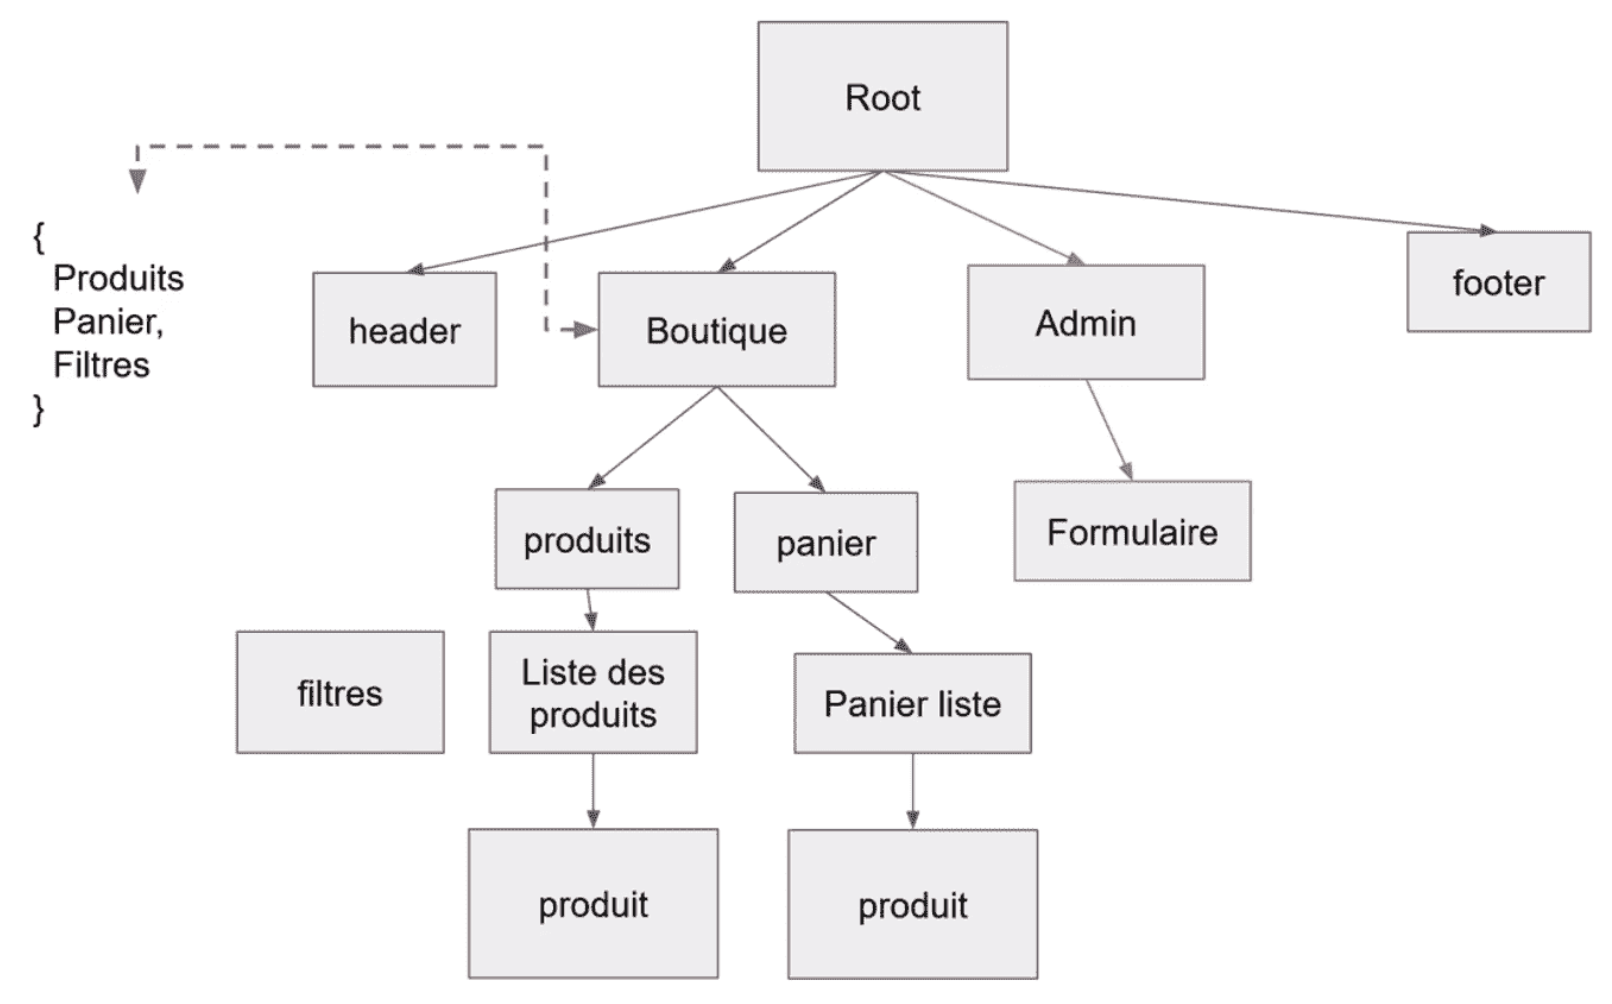
\includegraphics[width=10cm]{images/image33.png}
\end{center}

Notez que l'état des produits, du panier et des filtres sera contenu dans le composant Boutique.

\subsection{Création de nouveaux dossiers}
Dans le dossier srccréez un dossier features.

Dans ce dossier, créez les dossiers boutiqueet admin.

Dans le dossier boutiquecréez un dossier components. Déplacez-y les dossiers Cartet Shop.

Créez également dans boutiqueun dossier dataet un fichier Boutique.vue.

\subsection{Modification de App.vue}
La plupart de la logique dans le composant racine est déplacée dans le composant Boutique, nous n'avons donc plus que :
\begin{minted}[
mathescape,
framesep=2mm,
baselinestretch=1.2,
fontsize=\footnotesize,
bgcolor=LightGray,
%linenos
]{html}
<script setup lang="ts">
import TheHeader from './components/Header.vue';
import TheFooter from './components/Footer.vue';
import Boutique from './features/boutique/Boutique.vue';
</script>

<template>
  <div class="app-container">
    <TheHeader class="header" />
    <div class="app-content"><Component :is="Boutique" /></div>
    <TheFooter class="footer" />
  </div>
</template>

<style lang="scss">
@import './assets/scss/base.scss';
@import './assets/scss/debug.scss';

.app-container {
  min-height: 100vh;
  display: grid;
  grid-template-areas: 'header' 'app-content' 'footer';
  grid-template-rows: 48px auto 48px;
}

.header {  grid-area: header;}
.app-content {  grid-area: app-content;}
.footer {  grid-area: footer;}
</style>
\end{minted}

Notez bien l'utilisation du composant dynamique qui nous permettra de changer le composant affiché.

\subsection{Modification de Boutique.vue}
Voici le composant Boutiqueaprès y avoir déplacé toute la logique relative à la boutique :
\begin{minted}[
mathescape,
framesep=2mm,
baselinestretch=1.2,
fontsize=\footnotesize,
bgcolor=LightGray,
%linenos
]{html}
<script setup lang="ts">
import Shop from './components/Shop/Shop.vue';
import Cart from './components/Cart/Cart.vue';
import data from '../../data/product';
import { computed, reactive } from 'vue';
import type {
  FiltersInterface,
  ProductCartInterface,
  ProductInterface,
  FilterUpdate,
} from '../../interfaces';
import { DEFAULT_FILTERS } from '../../data/filters';

const state = reactive<{
  products: ProductInterface[];
  cart: ProductCartInterface[];
  filters: FiltersInterface;
}>({
  products: data,
  cart: [],
  filters: { ...DEFAULT_FILTERS },
});

function addProductToCart(productId: number): void {
  const product = state.products.find((product) => product.id === productId);
  if (product) {
    const productInCart = state.cart.find(
      (product) => product.id === productId
    );
    if (productInCart) {
      productInCart.quantity++;
    } else {
      state.cart.push({ ...product, quantity: 1 });
    }
  }
}

function removeProductFromCart(productId: number): void {
  const productFromCart = state.cart.find(
    (product) => product.id === productId
  );
  if (productFromCart?.quantity === 1) {
    state.cart = state.cart.filter((product) => product.id !== productId);
  } else {
    productFromCart.quantity--;
  }
}

function updateFilter(filterUpdate: FilterUpdate) {
  if (filterUpdate.search !== undefined) {
    state.filters.search = filterUpdate.search;
  } else if (filterUpdate.priceRange) {
    state.filters.priceRange = filterUpdate.priceRange;
  } else if (filterUpdate.category) {
    state.filters.category = filterUpdate.category;
  } else {
    state.filters = { ...DEFAULT_FILTERS };
  }
}

const cartEmpty = computed(() => state.cart.length === 0);

const filteredProducts = computed(() => {
  return state.products.filter((product) => {
    if (
      product.title
        .toLocaleLowerCase()
        .startsWith(state.filters.search.toLocaleLowerCase()) &&
      product.price >= state.filters.priceRange[0] &&
      product.price <= state.filters.priceRange[1] &&
      (product.category === state.filters.category ||
        state.filters.category === 'all')
    ) {
      return true;
    } else {
      return false;
    }
  });
});
</script>

<template>
  <div class="boutique-container" :class="{ 'grid-empty': cartEmpty }">
    <Shop
      @update-filter="updateFilter"
      :products="filteredProducts"
      :filters="state.filters"
      @add-product-to-cart="addProductToCart"
      class="shop"
    />
    <Cart
      v-if="!cartEmpty"
      :cart="state.cart"
      class="cart"
      @remove-product-from-cart="removeProductFromCart"
    />
  </div>
</template>

<style lang="scss">
.boutique-container {
  display: grid;
  grid-template-columns: 75% 25%;
}
.grid-empty {
  grid-template-columns: 100%;
}
.cart {
  background-color: white;
  border-left: var(--border);
}
</style>
\end{minted}

Code de la vidéo
Voici le code de la vidéo :
%%%%%%%%%%%%%%%%%%%%%%%%%%%%%%%%%%%%%%%%%%%%%%%%%%%%%%%%%%%%%%%%%%

\section{Navigation à l'aide d'un composant dynamique}
\subsection{Création du composant {\tt Admin}}
Dans le dossier {\tt src/features/admin} créer le composant {\color{monOrange}Admin.vue}:
\begin{minted}[
mathescape,
framesep=2mm,
baselinestretch=1.2,
fontsize=\footnotesize,
bgcolor=LightGray,
%linenos
]{html}
<script setup lang="ts"></script>

<template></template>

<style scoped lang="scss"></style>
\end{minted}
\subsection{Création du fichier {\tt type.ts}}
Dans le dossier {\color{monOrange}interfaces} créé le fichier {\tt type.ts} qui va contenir nos types littéraires :
\begin{minted}[
mathescape,
framesep=2mm,
baselinestretch=1.2,
fontsize=\footnotesize,
bgcolor=LightGray,
%linenos
]{html}
export type Page = 'Boutique' | 'Admin';
export type Category = 'gamer' | 'desktop' | 'streaming' | 'all';
\end{minted}
N'oubliez pas de modifier le fichier {\tt index.ts} dans le même dossier :
\begin{minted}[
mathescape,
framesep=2mm,
baselinestretch=1.2,
fontsize=\footnotesize,
bgcolor=LightGray,
%linenos
]{html}
export * from './Product.interface';
export * from './ProductCart.interface';
export * from './Filters.interface';
export * from './type';
\end{minted}
Ainsi que l'import dans {\tt Filters.interface.ts} et {\tt Product.interface.ts}:
\begin{minted}[
mathescape,
framesep=2mm,
baselinestretch=1.2,
fontsize=\footnotesize,
bgcolor=LightGray,
%linenos
]{html}
import type { Category } from './type';
\end{minted}
\subsection{Modification de {\tt App.vue}}
Dans le composant {\color{monOrange}App.vue} nous allons mettre en place les deux composants possibles dans le composant dynamique et la navigation entre les deux :
\begin{minted}[
mathescape,
framesep=2mm,
baselinestretch=1.2,
fontsize=\footnotesize,
bgcolor=LightGray,
%linenos
]{html}
<script setup lang="ts">
import TheHeader from './components/Header.vue';
import TheFooter from './components/Footer.vue';
import Boutique from './features/boutique/Boutique.vue';
import Admin from './features/admin/Admin.vue';
import { reactive, type Component as C } from 'vue';
import type { Page } from './interfaces';

const state = reactive<{
    page: Page
}>({
    page: 'Boutique'
})

const pages: { [s: string]: C } = {
    Boutique,
    Admin
}

function navigate(page: Page): void {
    state.page = page;
}
</script>

<template>
  <div class="app-container">
    <TheHeader @navigate="navigate" :page="state.page" class="header" />
    <div class="app-content">
      <Component :is="pages[state.page]" />
    </div>
    <TheFooter class="footer" />
  </div>
</template>

<style lang="scss">
@use './assets/scss/base.scss' as *;
@use './assets/scss/debug.scss' as *;

.app-container {
  min-height: 100vh;
  display: grid;
  grid-template-areas: 'header' 'app-content' 'footer';
  grid-template-rows: 48px auto 48px;
}

.header {
  grid-area: header;
}

.app-content {
  grid-area: app-content;
}

.footer {
  grid-area: footer;
}
</style>
\end{minted}
\subsection{Modification de {\tt Header.vue}}
Nous utilisons l'événement et la {\color{monOrange}props} définition dans le composant racine afin de pouvoir naviguer entre les composants {\color{monOrange}Admin} et {\color{monOrange}Boutique}:
\begin{minted}[
mathescape,
framesep=2mm,
baselinestretch=1.2,
fontsize=\footnotesize,
bgcolor=LightGray,
%linenos
]{html}
<script setup lang="ts">
import type { Page } from '@/interfaces';
defineProps<{
  page: Page;
}>();
const emit = defineEmits<{
  (e: 'navigate', page: Page): void;
}>();
</script>

<template>
  <header class="px-20 d-flex flex-row align-items-center">
    <a href="#" class="d-flex flex-row align-items-center mr-20">
      <img
        src="https://upload.wikimedia.org/wikipedia/commons/9/95/Vue.js_Logo_2.svg"
      />
      <span class="logo">Dyma</span>
    </a>
    <ul class="d-flex flex-row flex-fill">
      <li class="mr-10">
        <a
          :class="{ active: page === 'Boutique' }"
          @click="emit('navigate', 'Boutique')"
          >Boutique</a
        >
      </li>
      <li>
        <a
          :class="{ active: page === 'Admin' }"
          @click="emit('navigate', 'Admin')"
          >Admin</a
        >
      </li>
    </ul>
    <ul class="d-flex flex-row">
      <li class="mr-10">
        <a href="#">Inscription</a>
      </li>
      <li>
        <a href="#">Connexion</a>
      </li>
    </ul>
  </header>
</template>

<style lang="scss" scoped>
header {
  background-color: var(--primary-1);
  a {
    color: var(--text-primary-color);
    img {
      width: 20px;
      margin-right: 5px;
    }
    .logo {
      font-weight: 700;
      font-size: 20px;
    }
  }
  a.active {
    text-decoration: underline;
  }
}
</style>
\end{minted}
\subsection{Modification de {\tt src/assets/scss/base.scss}}
Ajoutez une classe pour nos cartes :
\begin{minted}[
mathescape,
framesep=2mm,
baselinestretch=1.2,
fontsize=\footnotesize,
bgcolor=LightGray,
%linenos
]{html}
.card {
    border: var(--border);
    border-radius: var(--border-radius);
    background-color:white;
    padding: 30px;
}
\end{minted}
\subsection{Création du composant {\tt ProductForm}}
Dans le dossier {\tt features/admin} créez un dossier {\color{monOrange}components} dans lequel vous mettez le fichier {\tt ProductForm.vue}:
\begin{minted}[
mathescape,
framesep=2mm,
baselinestretch=1.2,
fontsize=\footnotesize,
bgcolor=LightGray,
%linenos
]{html}
<script setup lang="ts"></script>

<template>
  <div class="card">
    <h1>Formulaire</h1>
  </div>
</template>

<style scoped lang="scss">
.card {
  width: 100%;
  max-width: 500px;
}
</style>
\end{minted}
\subsection{Modification du composant {\tt Admin}}
Nous utilisons ce composant dans le composant {\color{monOrange}Admin.vue}:
\begin{minted}[
mathescape,
framesep=2mm,
baselinestretch=1.2,
fontsize=\footnotesize,
bgcolor=LightGray,
%linenos
]{html}
<script setup lang="ts">
import ProductForm from './components/ProductForm.vue';
</script>

<template>
  <div
    class="
      admin-container
      d-flex
      flex-row
      justify-content-center
      align-items-center
    "
  >
    <ProductForm />
  </div>
</template>

<style scoped lang="scss">
.admin-container {
  height: 100%;
}
</style>
\end{minted}
%Code de la vidéo
%Voici le code de la vidéo :

\begin{center}
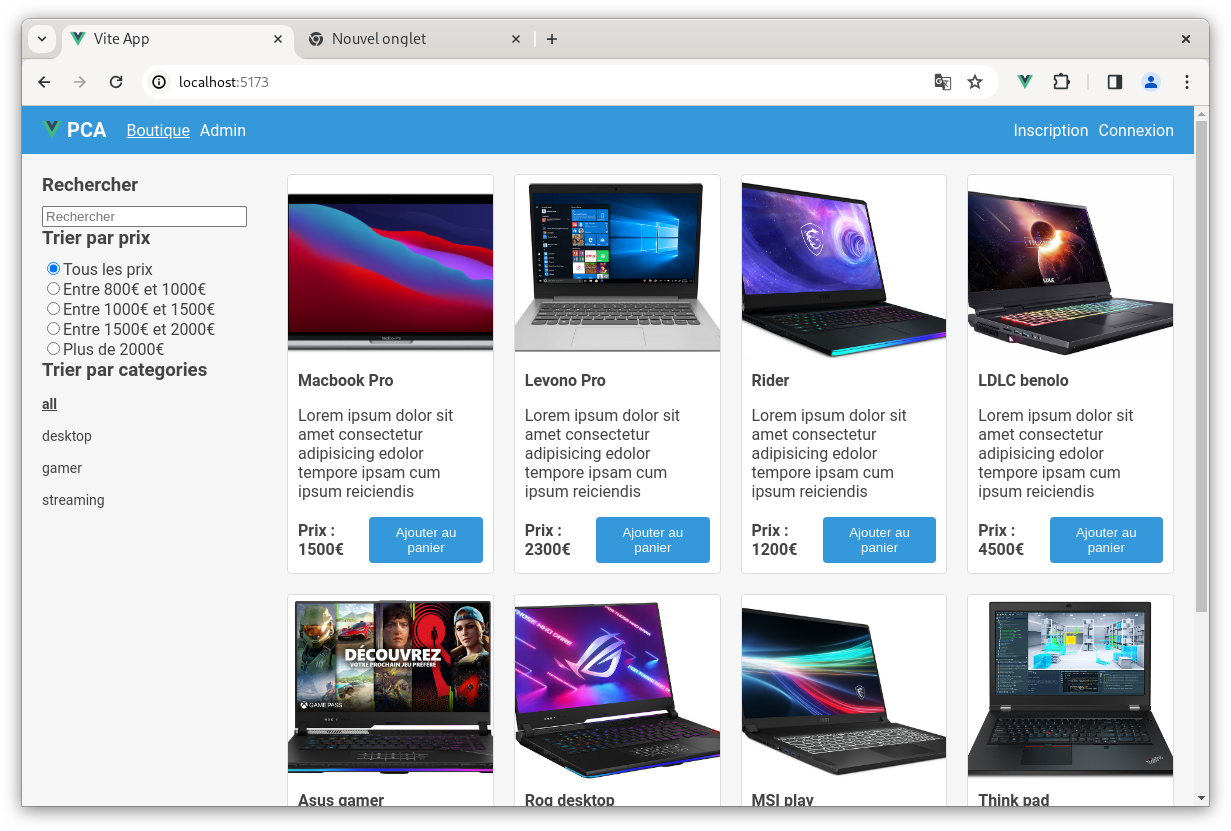
\includegraphics[width=12cm]{images/image34.png}
\end{center}

%%%%%%%%%%%%%%%%%%%%%%%%%%%%%%%%%%%%%%%%%%%%%%%%%%%%

\section{Mise en place du formulaire}
\subsection{Modification {\color{monOrange}debase.scss}}
Ajoutez les classes suivantes pour le formulaire :
\begin{minted}[
mathescape,
framesep=2mm,
baselinestretch=1.2,
fontsize=\footnotesize,
bgcolor=LightGray,
%linenos
]{html}
input, textarea, select {
    border: var(--border);
    border-radius: var(--border-radius);
    padding: 8px 15px;
}

label {
    font-size: 14px;
    font-weight: 500;
    color: var(--gray-3);
}

.form-error {
    color: var(--danger-1);
    font-size: 14px;
    font-weight: 500;
}
\end{minted}
\subsection{Modification de {\color{monOrange}ProductForm.vue}}
Nous mettons en place le formulaire et la validation :
\begin{minted}[
mathescape,
framesep=2mm,
baselinestretch=1.2,
fontsize=\footnotesize,
bgcolor=LightGray,
%linenos
]{html}
<script setup lang="ts">
import { useForm, useField } from 'vee-validate';
import { z } from 'zod';
import { toTypedSchema } from '@vee-validate/zod';

const required = { required_error: 'Veuillez renseigner ce champ' };
const validationSchema = toTypedSchema(
  z.object({
    title: z
      .string(required)
      .min(1, { message: 'Le titre doit faire au moins 1 caractère' })
      .max(20, { message: 'Le titre doit faire moins de 20 caractères' }),
    image: z.string(required),
    price: z
      .number(required)
      .min(0, { message: 'Le prix doit être supérieur à 0€' })
      .max(15000, { message: 'Le prix doit être inférieur à 150 00€' }),
    description: z
      .string(required)
      .min(10, { message: 'La description doit faire au moins 10 caractères' }),
    category: z.string(required),
  })
);

const { handleSubmit, isSubmitting } = useForm({
  validationSchema,
});

const title = useField('title');
const image = useField('image');
const price = useField('price');
const description = useField('description');
const category = useField('category');

const trySubmit = handleSubmit((formValues) => {
  console.log(formValues);
});
</script>

<template>
  <div class="card">
    <h3 class="mb-10">Ajouter un article</h3>
    <form @submit="trySubmit">
      <div class="d-flex flex-column mb-20">
        <label class="mb-5">*Titre</label>
        <input v-model="title.value.value" type="text" />
        <small class="form-error" v-if="title.errorMessage.value">{{
          title.errorMessage.value
        }}</small>
      </div>
      <div class="d-flex flex-column mb-20">
        <label class="mb-5">*Image</label>
        <input v-model="image.value.value" type="text" />
        <small class="form-error" v-if="image.errorMessage.value">{{
          image.errorMessage.value
        }}</small>
      </div>
      <div class="d-flex flex-column mb-20">
        <label class="mb-5">*Prix</label>
        <input v-model="price.value.value" type="number" />
        <small class="form-error" v-if="price.errorMessage.value">{{
          price.errorMessage.value
        }}</small>
      </div>
      <div class="d-flex flex-column mb-20">
        <label class="mb-5">*Description</label>
        <textarea v-model="(description.value.value as string)"></textarea>
        <small class="form-error" v-if="description.errorMessage.value">{{
          description.errorMessage.value
        }}</small>
      </div>
      <div class="d-flex flex-column mb-20">
        <label class="mb-5">*Catégorie</label>
        <select v-model="category.value.value">
          <option value disabled>Choisissez une catégorie</option>
          <option value="gamer">Jeu</option>
          <option value="desktop">Bureautique</option>
          <option value="streaming">Stream</option>
        </select>
        <small class="form-error" v-if="category.errorMessage.value">{{
          category.errorMessage.value
        }}</small>
      </div>
      <button class="btn btn-primary" :disabled="isSubmitting">
        Sauvegarder
      </button>
    </form>
  </div>
</template>

<style scoped lang="scss">
.card {
  width: 100%;
  max-width: 500px;
}
</style>
\end{minted}
{\tt image.value.value:} permet d'accéder à la propriété {\color{monOrange}value} retournée par {\color{monOrange}useField}, comme elle contient une {\color{monOrange}ref} qui est imbriquée dans l'objet, il n'y a pas d'accès automatique par {\color{monOrange}Vue} à la propriété {\color{monOrange}value} de la {\color{monOrange}ref} côté {\color{monOrange}template}( {\color{monOrange}unpacking}). Il faut donc y nous-mêmes.


%Code de la vidéo
%Voici le code de la vidéo :

\begin{center}
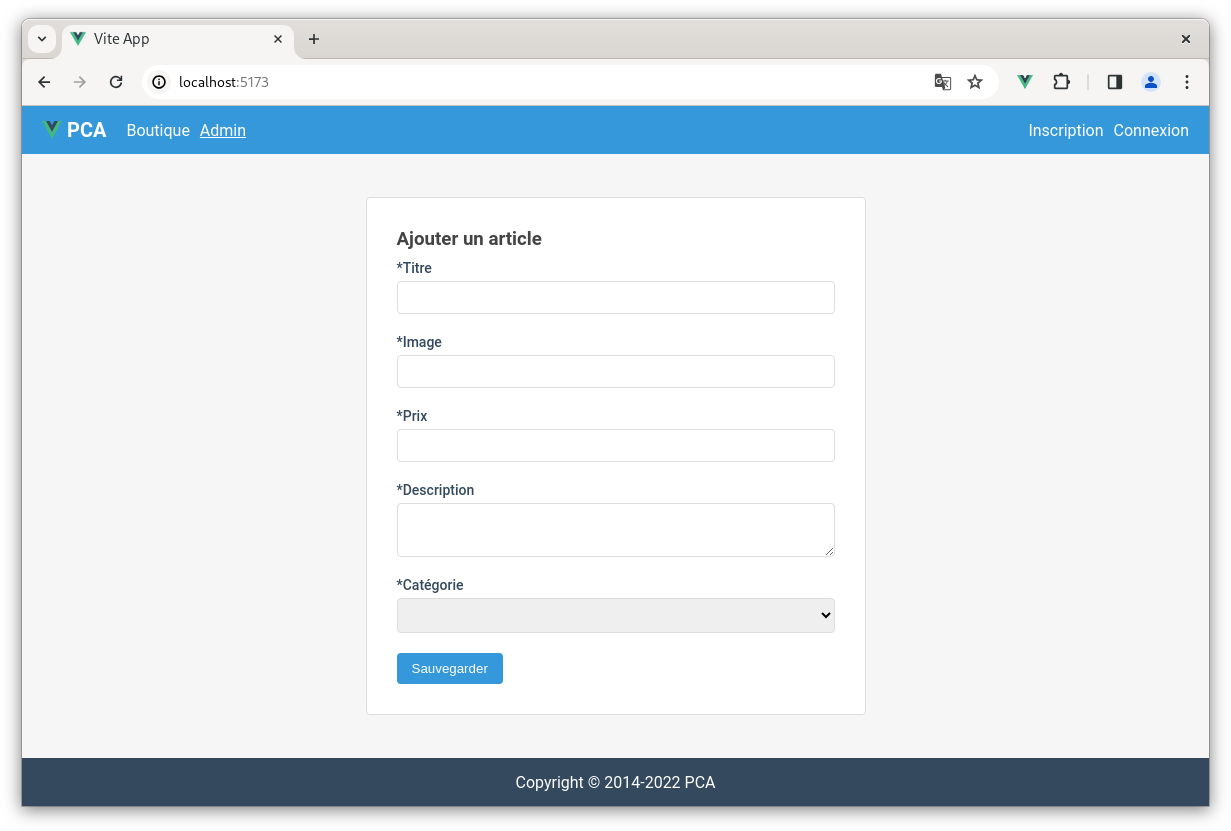
\includegraphics[width=12cm]{images/image35.png}
\end{center}

%%%%%%%%%%%%%%%%%%%%%%%%%%%%%%%%%%%%%%%%%%%%%%%%%%%%%%%

\section{Envoi du formulaire}
\subsection{Modification de {\color{monOrange}ProductForm.vue}}
Nous mettons en place l'envoi du formulaire au serveur {\color{monOrange}REST API}:
\begin{minted}[
mathescape,
framesep=2mm,
baselinestretch=1.2,
fontsize=\footnotesize,
bgcolor=LightGray,
%linenos
]{html}
<script setup lang="ts">
import { useForm, useField } from 'vee-validate';
import { z } from 'zod';
import { toTypedSchema } from '@vee-validate/zod';
import { onMounted, ref } from 'vue';

const firstInput = ref<HTMLInputElement | null>(null);
onMounted(() => {
  firstInput.value?.focus();
});

const required = { required_error: 'Veuillez renseigner ce champ' };
const validationSchema = toTypedSchema(
  z.object({
    title: z
      .string(required)
      .min(1, { message: 'Le titre doit faire au moins 1 caractère' })
      .max(20, { message: 'Le titre doit faire moins de 20 caractères' }),
    image: z.string(required),
    price: z
      .number(required)
      .min(0, { message: 'Le prix doit être supérieur à 0€' })
      .max(15000, { message: 'Le prix doit être inférieur à 150 00€' }),
    description: z
      .string(required)
      .min(10, { message: 'La description doit faire au moins 10 caractères' }),
    category: z.string(required),
  })
);

const { handleSubmit, isSubmitting } = useForm({
  validationSchema,
});

const title = useField('title');
const image = useField('image');
const price = useField('price');
const description = useField('description');
const category = useField('category');

const trySubmit = handleSubmit(async (formValues, { resetForm }) => {
  try {
    await fetch('https://restapi.fr/api/projetproducts', {
      method: 'POST',
      body: JSON.stringify(formValues),
      headers: {
        'Content-Type': 'application/json',
      },
    });
    resetForm();
    firstInput.value?.focus();
  } catch (e) {
    console.log(e);
  }
});
</script>

<template>
  <div class="card">
    <h3 class="mb-10">Ajouter un article</h3>
    <form @submit="trySubmit">
      <div class="d-flex flex-column mb-20">
        <label class="mb-5">*Titre</label>
        <input ref="firstInput" v-model="title.value.value" type="text" />
        <small class="form-error" v-if="title.errorMessage.value">{{
          title.errorMessage.value
        }}</small>
      </div>
      <div class="d-flex flex-column mb-20">
        <label class="mb-5">*Image</label>
        <input v-model="image.value.value" type="text" />
        <small class="form-error" v-if="image.errorMessage.value">{{
          image.errorMessage.value
        }}</small>
      </div>
      <div class="d-flex flex-column mb-20">
        <label class="mb-5">*Prix</label>
        <input v-model="price.value.value" type="number" />
        <small class="form-error" v-if="price.errorMessage.value">{{
          price.errorMessage.value
        }}</small>
      </div>
      <div class="d-flex flex-column mb-20">
        <label class="mb-5">*Description</label>
        <textarea v-model="(description.value.value as string)"></textarea>
        <small class="form-error" v-if="description.errorMessage.value">{{
          description.errorMessage.value
        }}</small>
      </div>
      <div class="d-flex flex-column mb-20">
        <label class="mb-5">*Catégorie</label>
        <select v-model="category.value.value">
          <option value disabled>Choisissez une catégorie</option>
          <option value="gamer">Jeu</option>
          <option value="desktop">Bureautique</option>
          <option value="streaming">Stream</option>
        </select>
        <small class="form-error" v-if="category.errorMessage.value">{{
          category.errorMessage.value
        }}</small>
      </div>
      <button class="btn btn-primary" :disabled="isSubmitting">
        Sauvegarder
      </button>
    </form>
  </div>
</template>

<style scoped lang="scss">
.card {
  width: 100%;
  max-width: 500px;
}
</style>
\end{minted}
\subsection{Modification de {\color{monOrange}Product.interface.ts}}
Nous modifions la propriété {\color{monOrange}id} car {\color{monOrange}MongoDB} (base de données utilisées pour la sauvegarde) utilisons la propriété {\color{monOrange}\_id} et nous ajoutons la propriété {\color{monOrange}createdAt} qui contient la date de création au format {\color{monOrange}ISO 8601}:
\begin{minted}[
mathescape,
framesep=2mm,
baselinestretch=1.2,
fontsize=\footnotesize,
bgcolor=LightGray,
%linenos
]{javascript}
import type { Category } from './type';

export interface ProductInterface {
  _id: string;
  createdAt: string;
  title: string;
  image: string;
  price: number;
  description: string;
  category: Category;
}
\end{minted}
\subsection{Création de {\tt src/data/seed.ts}}
Nous créons une fonction pour ajouter des données dans le service {\color{monOrange}restapi.fr} s'il n'y en a pas :
\begin{minted}[
mathescape,
framesep=2mm,
baselinestretch=1.2,
fontsize=\footnotesize,
bgcolor=LightGray,
%linenos
]{javascript}
import data from './product';

export async function seed(collectionName: string) {
  await fetch(`https://restapi.fr/api/${collectionName}`, {
    method: 'POST',
    body: JSON.stringify(data),
    headers: {
      'Content-Type': 'application/json',
    },
  });
}
\end{minted}
%$
\subsection{Modification de {\color{monOrange}App.vue}}
Nous appelons notre fonction permettant d'enregistrer nos données initiales, n'oubliez pas de la commenter après l'avoir exécuté une fois :
\begin{minted}[
mathescape,
framesep=2mm,
baselinestretch=1.2,
fontsize=\footnotesize,
bgcolor=LightGray,
%linenos
]{html}
<script setup lang="ts">
import TheHeader from './components/Header.vue';
import TheFooter from './components/Footer.vue';
import Boutique from './features/boutique/Boutique.vue';
import Admin from './features/admin/Admin.vue';
import { reactive, type Component as C } from 'vue';
import type { Page } from './interfaces';
import { seed } from './data/seed';

const state = reactive<{
    page: Page
}>({
    page: 'Boutique'
})

const pages: { [s: string]: C } = {
    Boutique,
    Admin
}

function navigate(page: Page): void {
    state.page = page;
}

// seed('projetproducts'); N’oubliez pas de commenter !
</script>

<template>
  <div class="app-container">
    <TheHeader @navigate="navigate" :page="state.page" class="header" />
    <div class="app-content">
      <Component :is="pages[state.page]" />
    </div>
    <TheFooter class="footer" />
  </div>
</template>

<style lang="scss">
@use './assets/scss/base.scss' as *;
@use './assets/scss/debug.scss' as *;

.app-container {
  min-height: 100vh;
  display: grid;
  grid-template-areas: 'header' 'app-content' 'footer';
  grid-template-rows: 48px auto 48px;
}

.header {
  grid-area: header;
}

.app-content {
  grid-area: app-content;
}

.footer {
  grid-area: footer;
}
</style>
\end{minted}

\begin{center}
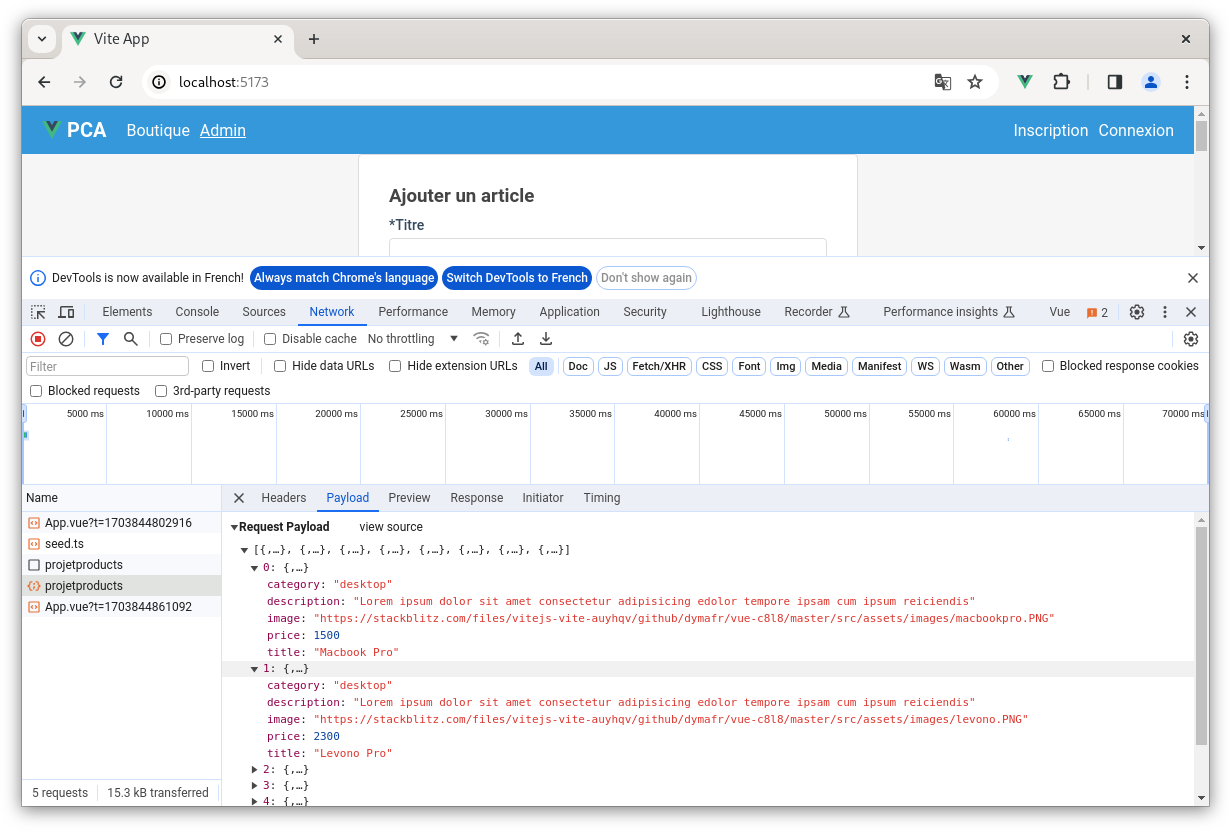
\includegraphics[width=12cm]{images/image36.png}
\end{center}

%%%%%%%%%%%%%%%%%%%%%%%%%%%%%%%%%%%%%%%%%%%%%%%%%%

\section{Récupération des produits}
\subsection{Modification de {\color{monOrange}Boutique.vue}}
Nous modifions le composant {\color{monOrange}Boutique} pour récupérer les produits :
\begin{minted}[
mathescape,
framesep=2mm,
baselinestretch=1.2,
fontsize=\footnotesize,
bgcolor=LightGray,
%linenos
]{html}
<script setup lang="ts">
import Shop from './components/Shop/Shop.vue';
import Cart from './components/Cart/Cart.vue';
import { computed, reactive } from 'vue';
import type {
  FiltersInterface,
  ProductCartInterface,
  ProductInterface,
  FilterUpdate,
} from '../../interfaces';
import { DEFAULT_FILTERS } from './data/filters';

const state = reactive<{
  products: ProductInterface[];
  cart: ProductCartInterface[];
  filters: FiltersInterface;
}>({
  products: [],
  cart: [],
  filters: { ...DEFAULT_FILTERS },
});

const products = await (
  await fetch('https://restapi.fr/api/projetproducts')
).json();
if (Array.isArray(products)) {
  state.products = products;
} else {
  state.products = [products];
}

function addProductToCart(productId: string): void {
  const product = state.products.find((product) => product._id === productId);
  if (product) {
    const productInCart = state.cart.find(
      (product) => product._id === productId
    );
    if (productInCart) {
      productInCart.quantity++;
    } else {
      state.cart.push({ ...product, quantity: 1 });
    }
  }
}

function removeProductFromCart(productId: string): void {
  const productFromCart = state.cart.find(
    (product) => product._id === productId
  );
  if (productFromCart?.quantity === 1) {
    state.cart = state.cart.filter((product) => product._id !== productId);
  } else {
    productFromCart.quantity--;
  }
}

function updateFilter(filterUpdate: FilterUpdate) {
  if (filterUpdate.search !== undefined) {
    state.filters.search = filterUpdate.search;
  } else if (filterUpdate.priceRange) {
    state.filters.priceRange = filterUpdate.priceRange;
  } else if (filterUpdate.category) {
    state.filters.category = filterUpdate.category;
  } else {
    state.filters = { ...DEFAULT_FILTERS };
  }
}

const cartEmpty = computed(() => state.cart.length === 0);

const filteredProducts = computed(() => {
  return state.products.filter((product) => {
    if (
      product.title
        .toLocaleLowerCase()
        .startsWith(state.filters.search.toLocaleLowerCase()) &&
      product.price >= state.filters.priceRange[0] &&
      product.price <= state.filters.priceRange[1] &&
      (product.category === state.filters.category ||
        state.filters.category === 'all')
    ) {
      return true;
    } else {
      return false;
    }
  });
});
</script>

<template>
  <div class="boutique-container" :class="{ 'grid-empty': cartEmpty }">
    <Shop
      @update-filter="updateFilter"
      :products="filteredProducts"
      :filters="state.filters"
      @add-product-to-cart="addProductToCart"
      class="shop"
    />
    <Cart
      v-if="!cartEmpty"
      :cart="state.cart"
      class="cart"
      @remove-product-from-cart="removeProductFromCart"
    />
  </div>
</template>

<style scoped lang="scss">
.boutique-container {
  display: grid;
  grid-template-columns: 75% 25%;
}
.grid-empty {
  grid-template-columns: 100%;
}
.cart {
  background-color: white;
  border-left: var(--border);
}
</style>
\end{minted}
Nous avons un {\color{monOrange}await} au premier niveau dans les balises {\color{monOrange}script} ce qui permet d'enregistrer ce composant comme ayant une dépendance asynchrone avec {\color{monOrange}Suspense}. N'oubliez pas de modifier l'utilisation des propriétés {\color{monOrange}id} par la propriété {\color{monOrange}\_id}.

\subsection{Modification de {\color{monOrange}App.vue}}
Nous utilisons Suspensepour attendre le chargement des produits :
\begin{minted}[
mathescape,
framesep=2mm,
baselinestretch=1.2,
fontsize=\footnotesize,
bgcolor=LightGray,
%linenos
]{html}
<template>
  <div class="app-container">
    <TheHeader @navigate="navigate" :page="state.page" class="header" />
    <div class="app-content">
      <Suspense>
        <Component :is="pages[state.page]" />
      </Suspense>
    </div>
    <TheFooter class="footer" />
  </div>
</template>
\end{minted}
\subsection{Modification du type de {\tt productId} et de la propriété {\tt id}}
Il faut modifier le type de {\color{monOrange}productId} en {\color{monOrange}string} et la propriété {\color{monOrange}id} des {\color{monOrange}products} par {\color{monOrange}\_id} dans les composants : {\color{monOrange}Shop.vue, ShopProductList.vue, ShopProduct.vue, Cart.vue, CartProductList.vue} et {\color{monOrange}CartProduct.vue}.

\begin{center}
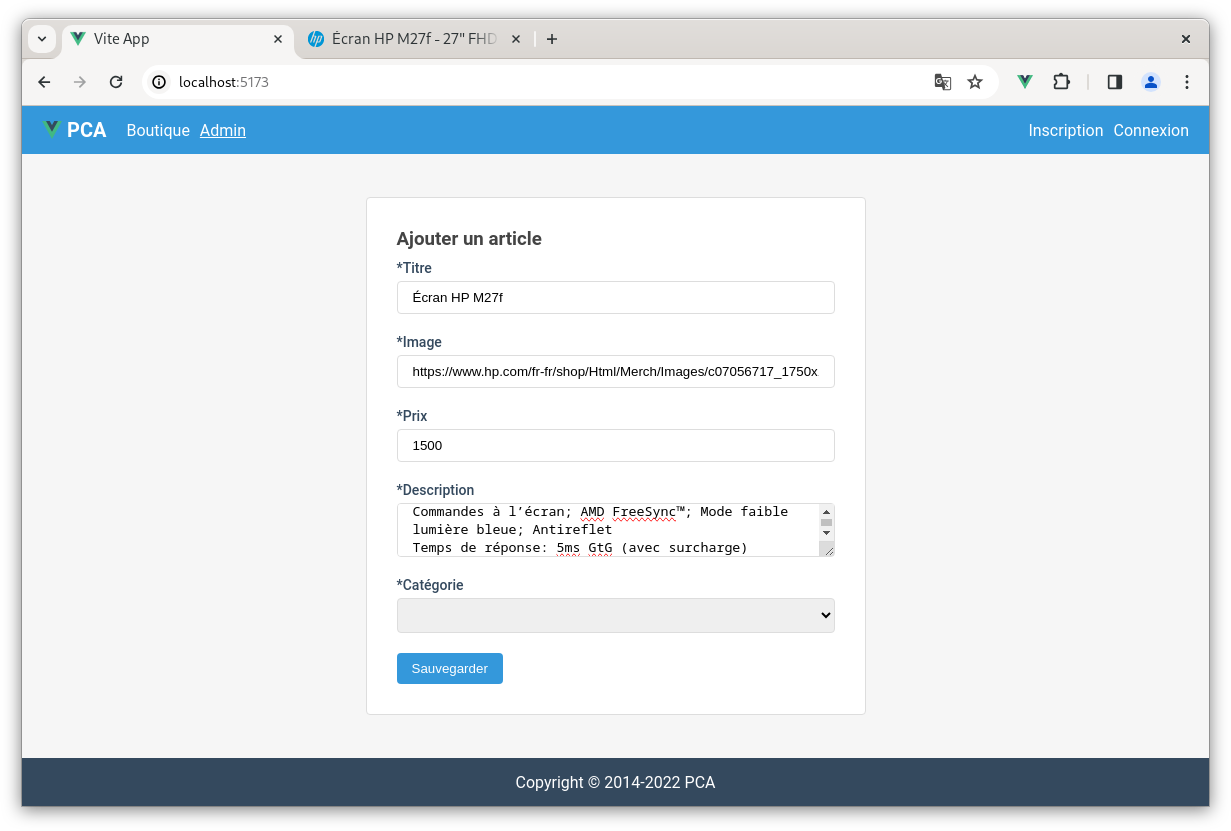
\includegraphics[width=10cm]{images/image37.png}
\end{center}

%%%%%%%%%%%%%%%%%%%%%%%%%%%%%%%%%%%%%%%%%%%%%%%%%%%%%%%%%%%%

\section{Amélioration du CSS}
\subsection{Modification de {\color{monOrange}App.vue}}
Modifiez le style du composant {\color{monOrange}App}:
\begin{minted}[
mathescape,
framesep=2mm,
baselinestretch=1.2,
fontsize=\footnotesize,
bgcolor=LightGray,
%linenos
]{html}
<style lang="scss">
@use './assets/scss/base.scss' as *;
@use './assets/scss/debug.scss' as *;

.app-container {
  height: 100vh;
  display: grid;
  grid-template-areas: 'header' 'app-content' 'footer';
  grid-template-rows: 48px auto 48px;
}

.header {
  grid-area: header;
}

.app-content {
  grid-area: app-content;
}

.footer {
  grid-area: footer;
}
</style>
\end{minted}
\subsection{Modification de {\color{monOrange}Shop.vue}}
Nous modifions le composant {\color{monOrange}Shop.vue} pour rendre {\color{monOrange}scrollable} la liste des produits :
\begin{minted}[
mathescape,
framesep=2mm,
baselinestretch=1.2,
fontsize=\footnotesize,
bgcolor=LightGray,
%linenos
]{html}
<script setup lang="ts">
import type {
  FiltersInterface,
  ProductInterface,
  FilterUpdate,
} from '../../interfaces';
import ShopProductList from './ShopProductList.vue';
import ShopFilters from './ShopFilters.vue';

defineProps<{
  products: ProductInterface[];
  filters: FiltersInterface;
}>();

const emit = defineEmits<{
  (e: 'addProductToCart', productId: string): void;
  (e: 'updateFilter', updateFilter: FilterUpdate): void;
}>();
</script>

<template>
  <div class="d-flex flex-row">
    <ShopFilters
      :filters="filters"
      :nbr-of-products="products.length"
      @update-filter="emit('updateFilter', $event)"
      class="shop-filter"
    />
    <ShopProductList
      class="flex-fill scrollable"
      @add-product-to-cart="emit('addProductToCart', $event)"
      :products="products"
    />
  </div>
</template>

<style lang="scss" scoped>
.scrollable {
  overflow-y: auto;
  height: calc(100vh - 96px);
}

.shop-filter {
  flex: 0 0 200px;
}
</style>
\end{minted}
\subsection{Création du fichier {\tt \_mixins.scss}}
Dans le dossier {\tt src/assets/scss} créez le fichier {\color{monOrange}\_mixins.scss}:
\begin{minted}[
mathescape,
framesep=2mm,
baselinestretch=1.2,
fontsize=\footnotesize,
bgcolor=LightGray,
%linenos
]{html}
@mixin sm {
  @media (min-width: 576px) {
    @content;
  }
}

@mixin md {
  @media (min-width: 768px) {
    @content;
  }
}

@mixin lg {
  @media (min-width: 992px) {
    @content;
  }
}

@mixin xl {
  @media (min-width: 1200px) {
    @content;
  }
}
\end{minted}
\subsection{Modification de {\color{monOrange}ShopProductList.vue}}
Nous utilisons nos {\color{monOrange}mixins} pour rendre la liste des produits {\color{monOrange}responsive} (c'est-à-dire qui s'adapte à la taille de l'écran) :
\begin{minted}[
mathescape,
framesep=2mm,
baselinestretch=1.2,
fontsize=\footnotesize,
bgcolor=LightGray,
%linenos
]{html}
<script setup lang="ts">
import type { ProductInterface } from '@/interfaces';
import ShopProduct from './ShopProduct.vue';

defineProps<{
  products: ProductInterface[];
}>();

const emit = defineEmits<{
  (e: 'addProductToCart', productId: string): void;
}>();
</script>

<template>
  <div class="grid p-20">
    <ShopProduct
      @add-product-to-cart="emit('addProductToCart', $event)"
      v-for="product of products"
      :product="product"
      :key="product._id"
    />
  </div>
</template>

<style lang="scss" scoped>
@use '../../../../assets/scss/mixins' as m;
.grid {
  display: grid;
  grid-template-columns: 1fr;
  @include m.md {
    grid-template-columns: 1fr 1fr;
  }
  @include m.lg {
    grid-template-columns: 1fr 1fr 1fr;
  }
  @include m.xl {
    grid-template-columns: 1fr 1fr 1fr 1fr;
  }
  grid-auto-rows: 400px;
  gap: 20px;
}
</style>
\end{minted}

%$
{\em Si vous ne comprenez pas le code revoyez les chapitres sur {\color{monOrange}Sass} et les {\color{monOrange}mixins} dans le cours {\color{monOrange}HTML \& CSS} .

\begin{center}
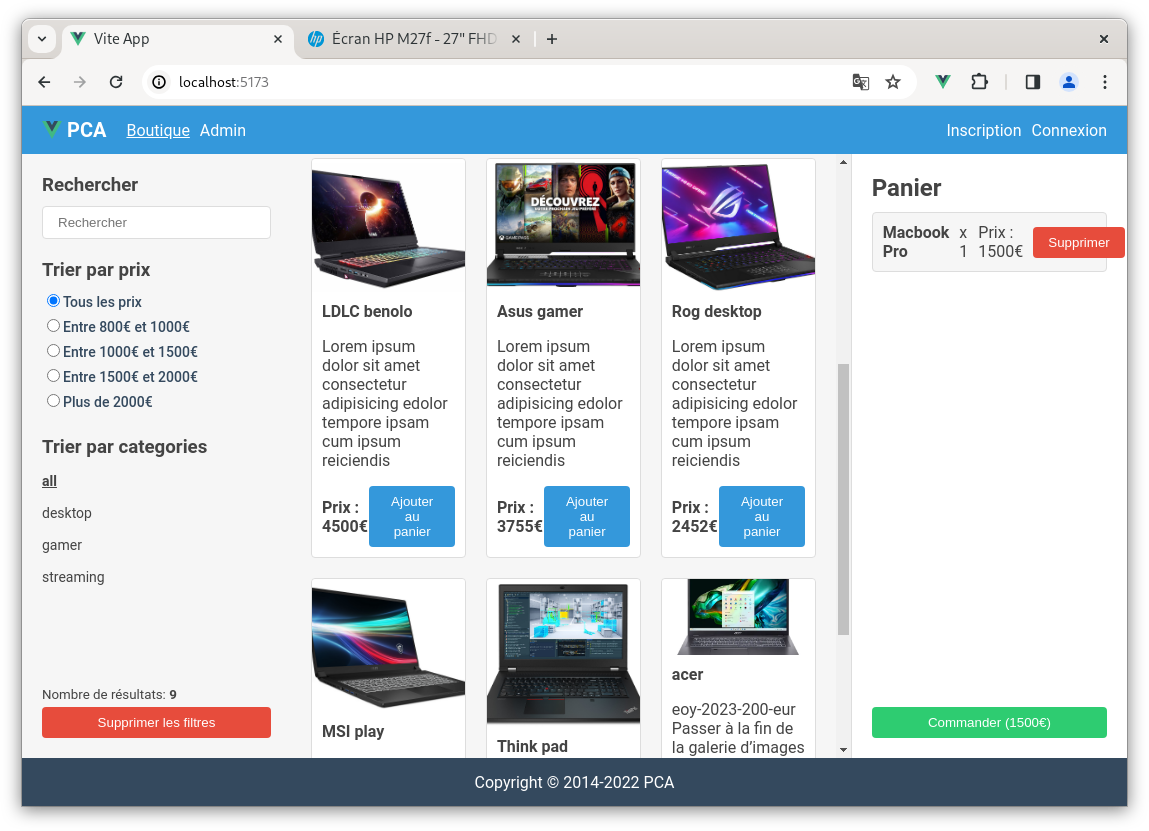
\includegraphics[width=10cm]{images/image38.png}
\end{center}
